\chapter{実験装置・手法[未完]\label{devicesection}}
\% 3Dプリンター作った治具によって, 内容も変わるので今のところは暫定の実験装置・手法です. 
\newpage
\section{概要}
本章では, ファントムに加振した際の1次元的なせん断波の伝播の様子をエコーパルスイメージングおよびリング型アレイトランスデューサ超音波CTで解析することで, ファントムの機械的特性を評価するものである. また, リング型アレイトランスデューサでは現段階ではリアルタイムで生体組織の挙動を観測することはできない. そのため, 各面内で得た断層画像から目的の生体組織を検出する方法についても検討する. また, ファントムの加振した際の挙動を記述する理論式を組み立てることで, 実験値と比較検討する.
\section{加振装置}
\figref{kashinsouchi}は, 本研究で使用した加振装置の概要である. 電圧で駆動させた振動モータを用いてファントムを振動させた. ファントムは弦などのごく細いもので, 一次元的な振動を与えた. 以下では, 加振装置の振動数の設定, ファントムの設定, 張力などの力学的条件の設定, バリデーションについて述べる. 
\begin{figure}[H]
  \begin{center}
    \includegraphics[width=110mm]{fig/jikkendevice.pdf}
  \end{center}
  \caption{加振装置}
  \figlab{kashinsouchi}
\end{figure}
%\begin{itemize}
\subsection{振動数の設定}
生体組織を振動させる方法としては手動, 音響放射圧, 機械的加振がある. その中でも, 機械的加振を選択したのは, 生体組織のより定量的な機械的特性の評価のためである. ファントムの振動手段としては振動モータを使用した. 実際に使用した振動モータを\figref{motor}に示す.
\begin{figure}[H]
  \begin{center}
    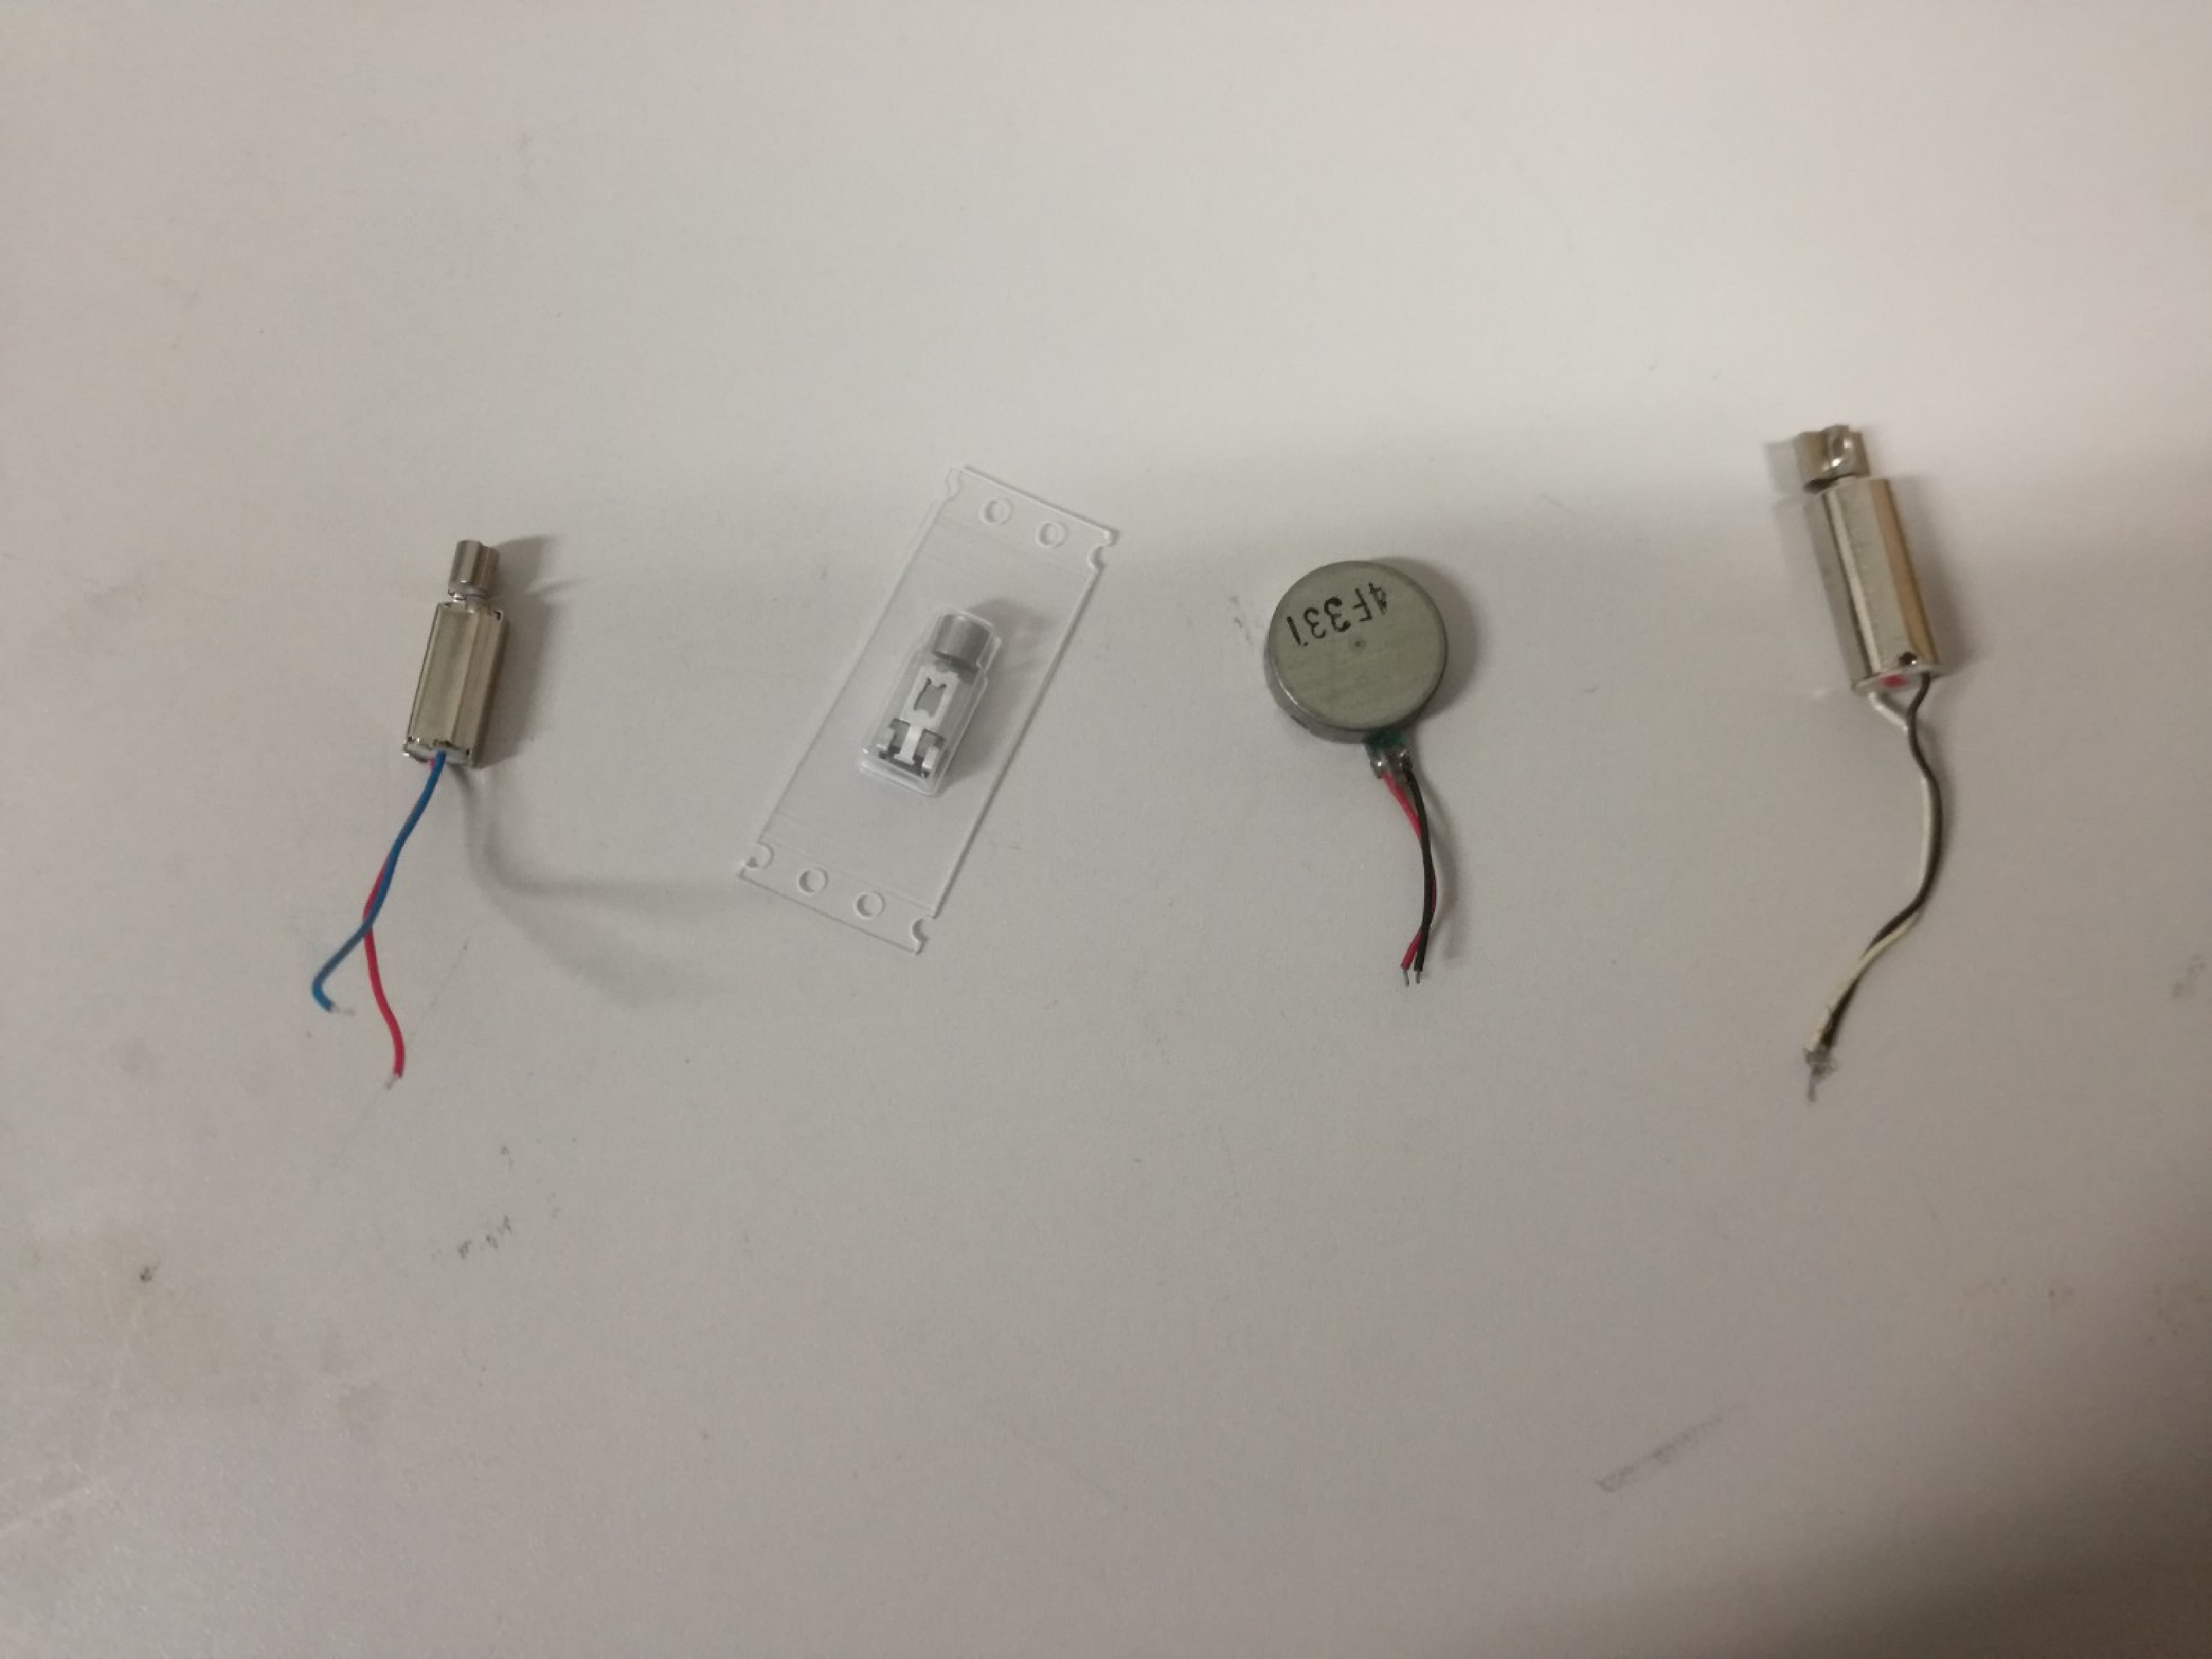
\includegraphics[width=70mm]{fig/motor.pdf}
  \end{center}
  \caption{振動モータ}
  \figlab{motor}
\end{figure}
振動モータ
\subsection{ファントムの設定}
本研究では, まずは釣り糸, 水糸のような強度や密度が規格化されているファントムを用いて計測した. その後に鳥の腱を用いて計測することで, 実際の生体組織に関しても本研究の生体組織の特性の定量かの妥当性を検討した. 実際に使用したファントムを\figref{fantom}に示す.
\begin{figure}[H]
  \begin{center}
    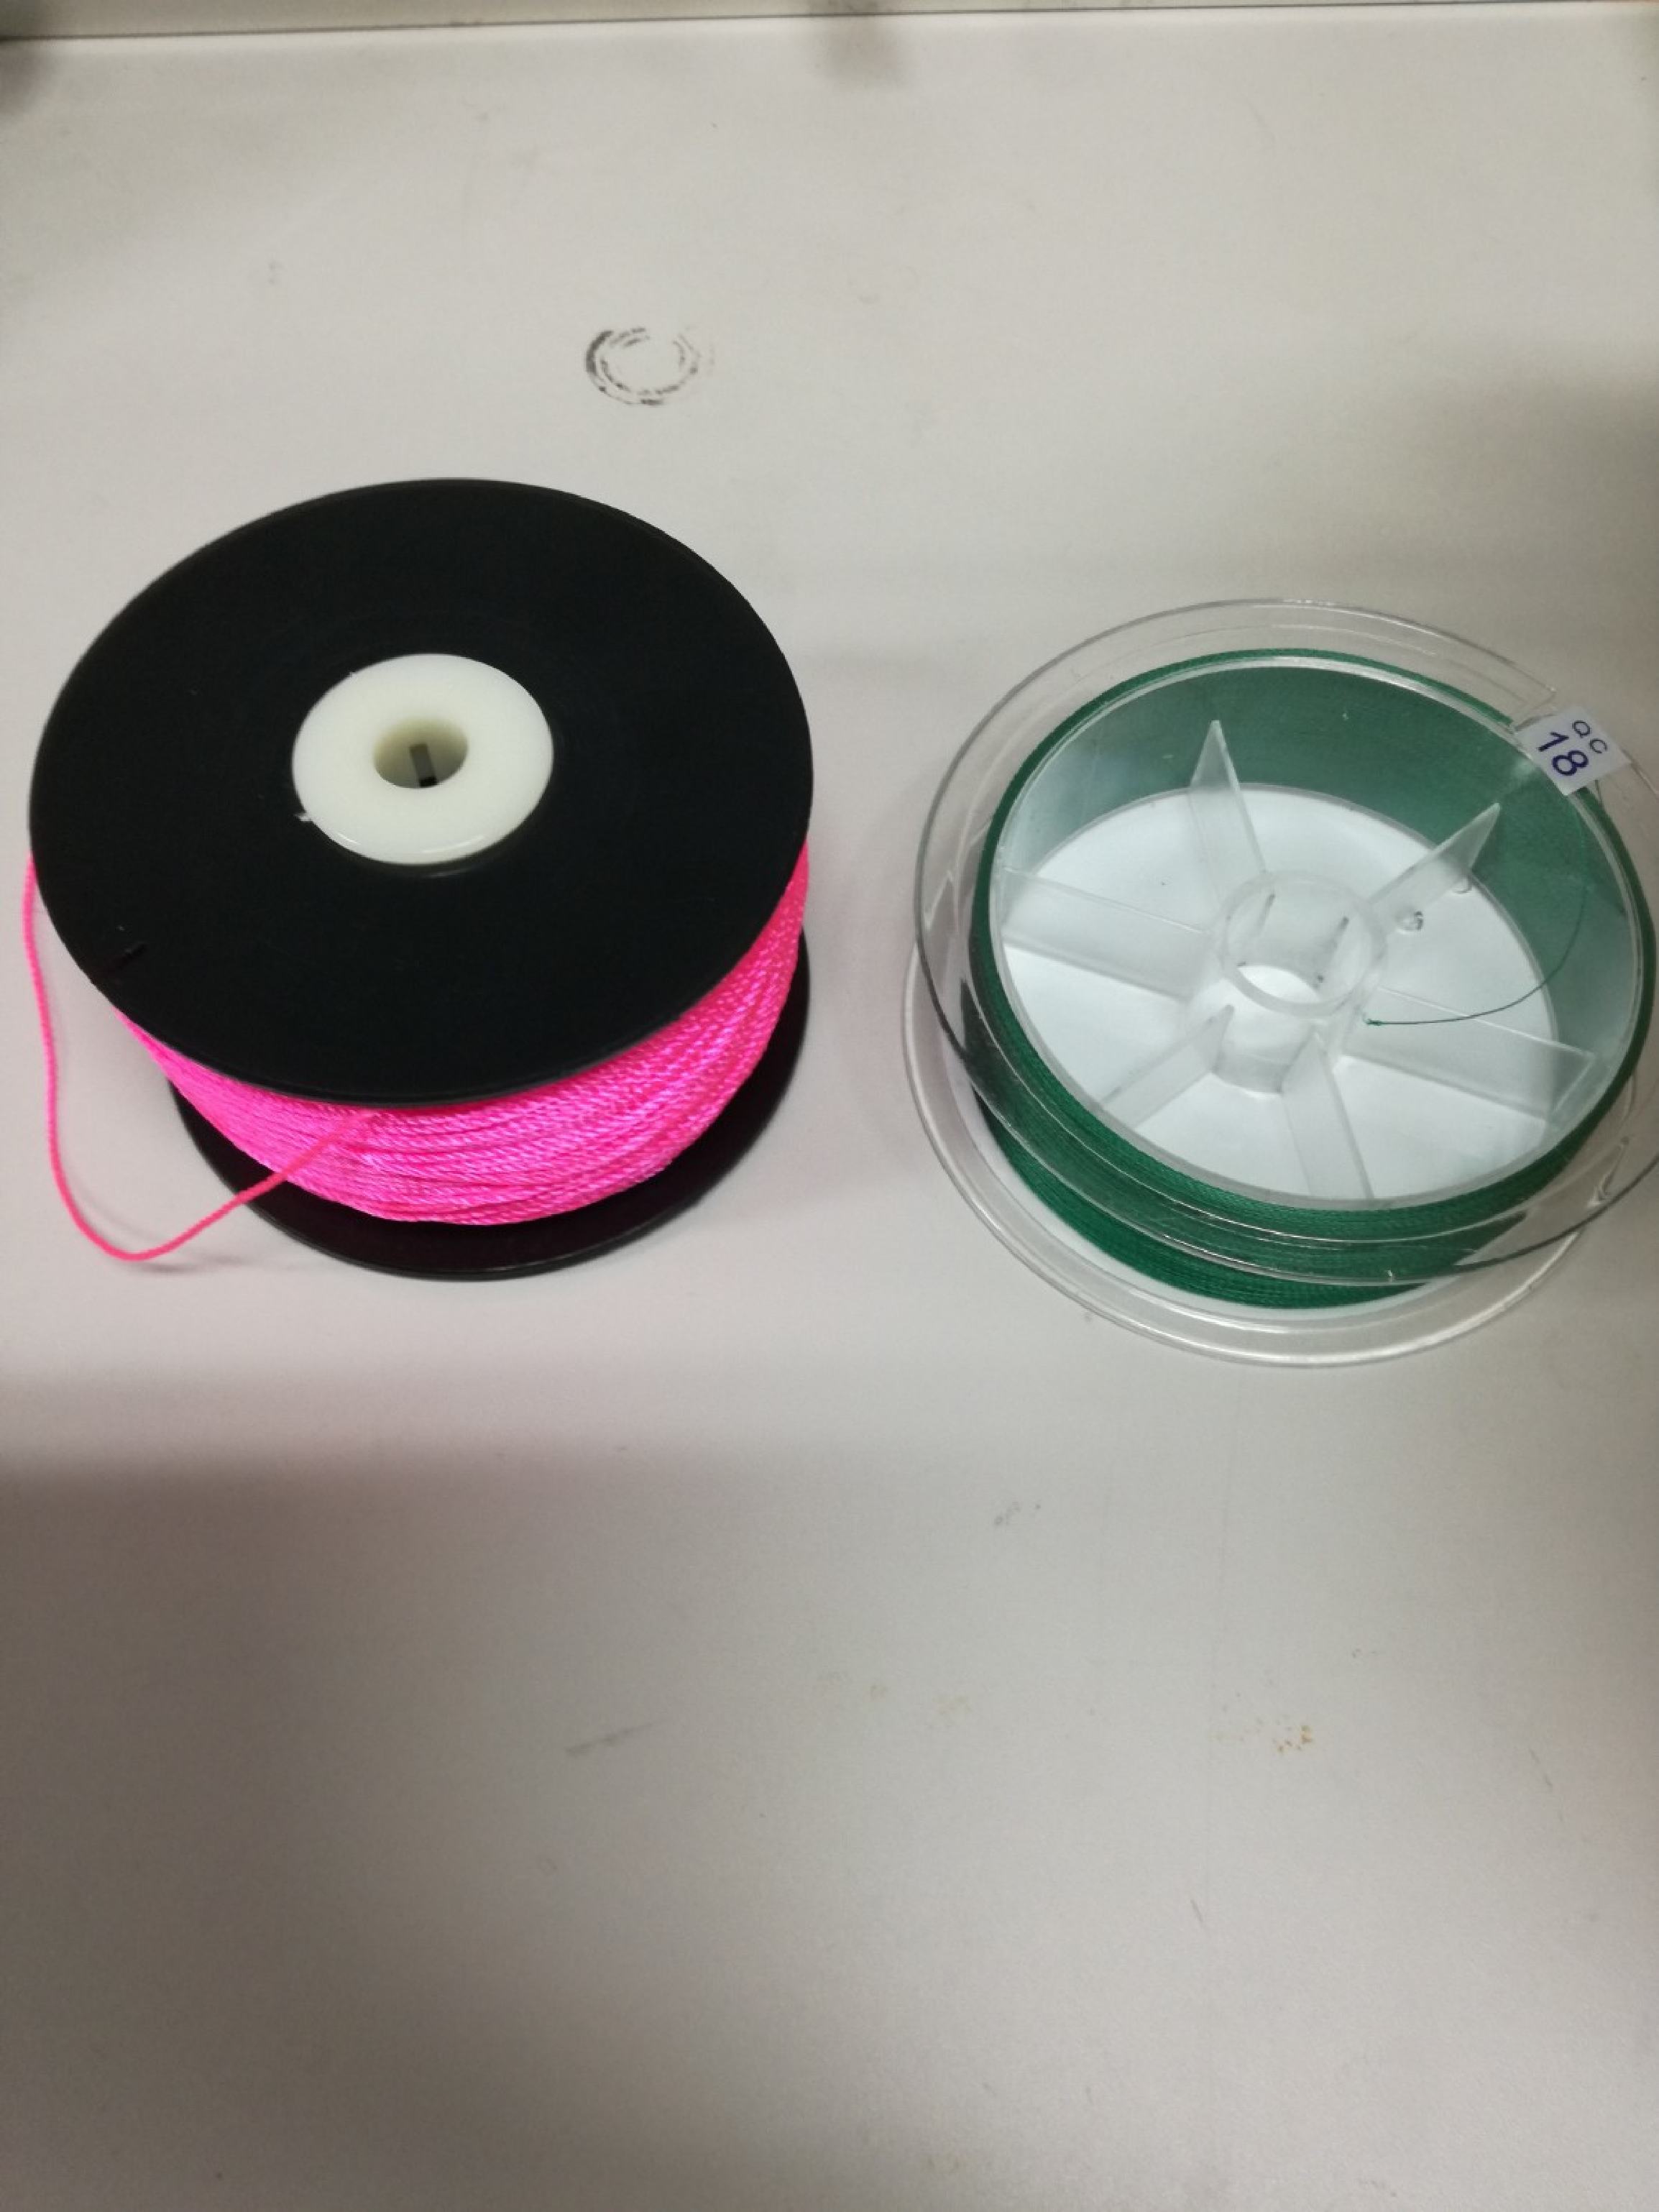
\includegraphics[width=30mm]{fig/fantom.pdf}
  \end{center}
  \caption{ファントム}
  \figlab{fantom}
\end{figure}
\subsection{力学的条件の設定}
\subsection{バリデーション}
カメラを用いて, ファントムを振動させた時のひずみを撮影する. 撮影した画像から, ひずみの伝播の様子を撮像し, RF信号から算出したひずみの伝播と定量的な比較をする. カメラの撮像の時間分解が, ファントムの振動に対して適切に設定される必要があるため, \figref{led}で示したLEDからストロボを作成し, 撮像の時間分解能を向上させる. LEDの挙動は, ファンクションジェネレータで駆動する. 
\begin{figure}[H]
 \begin{minipage}{0.5\hsize}
  \begin{center}
   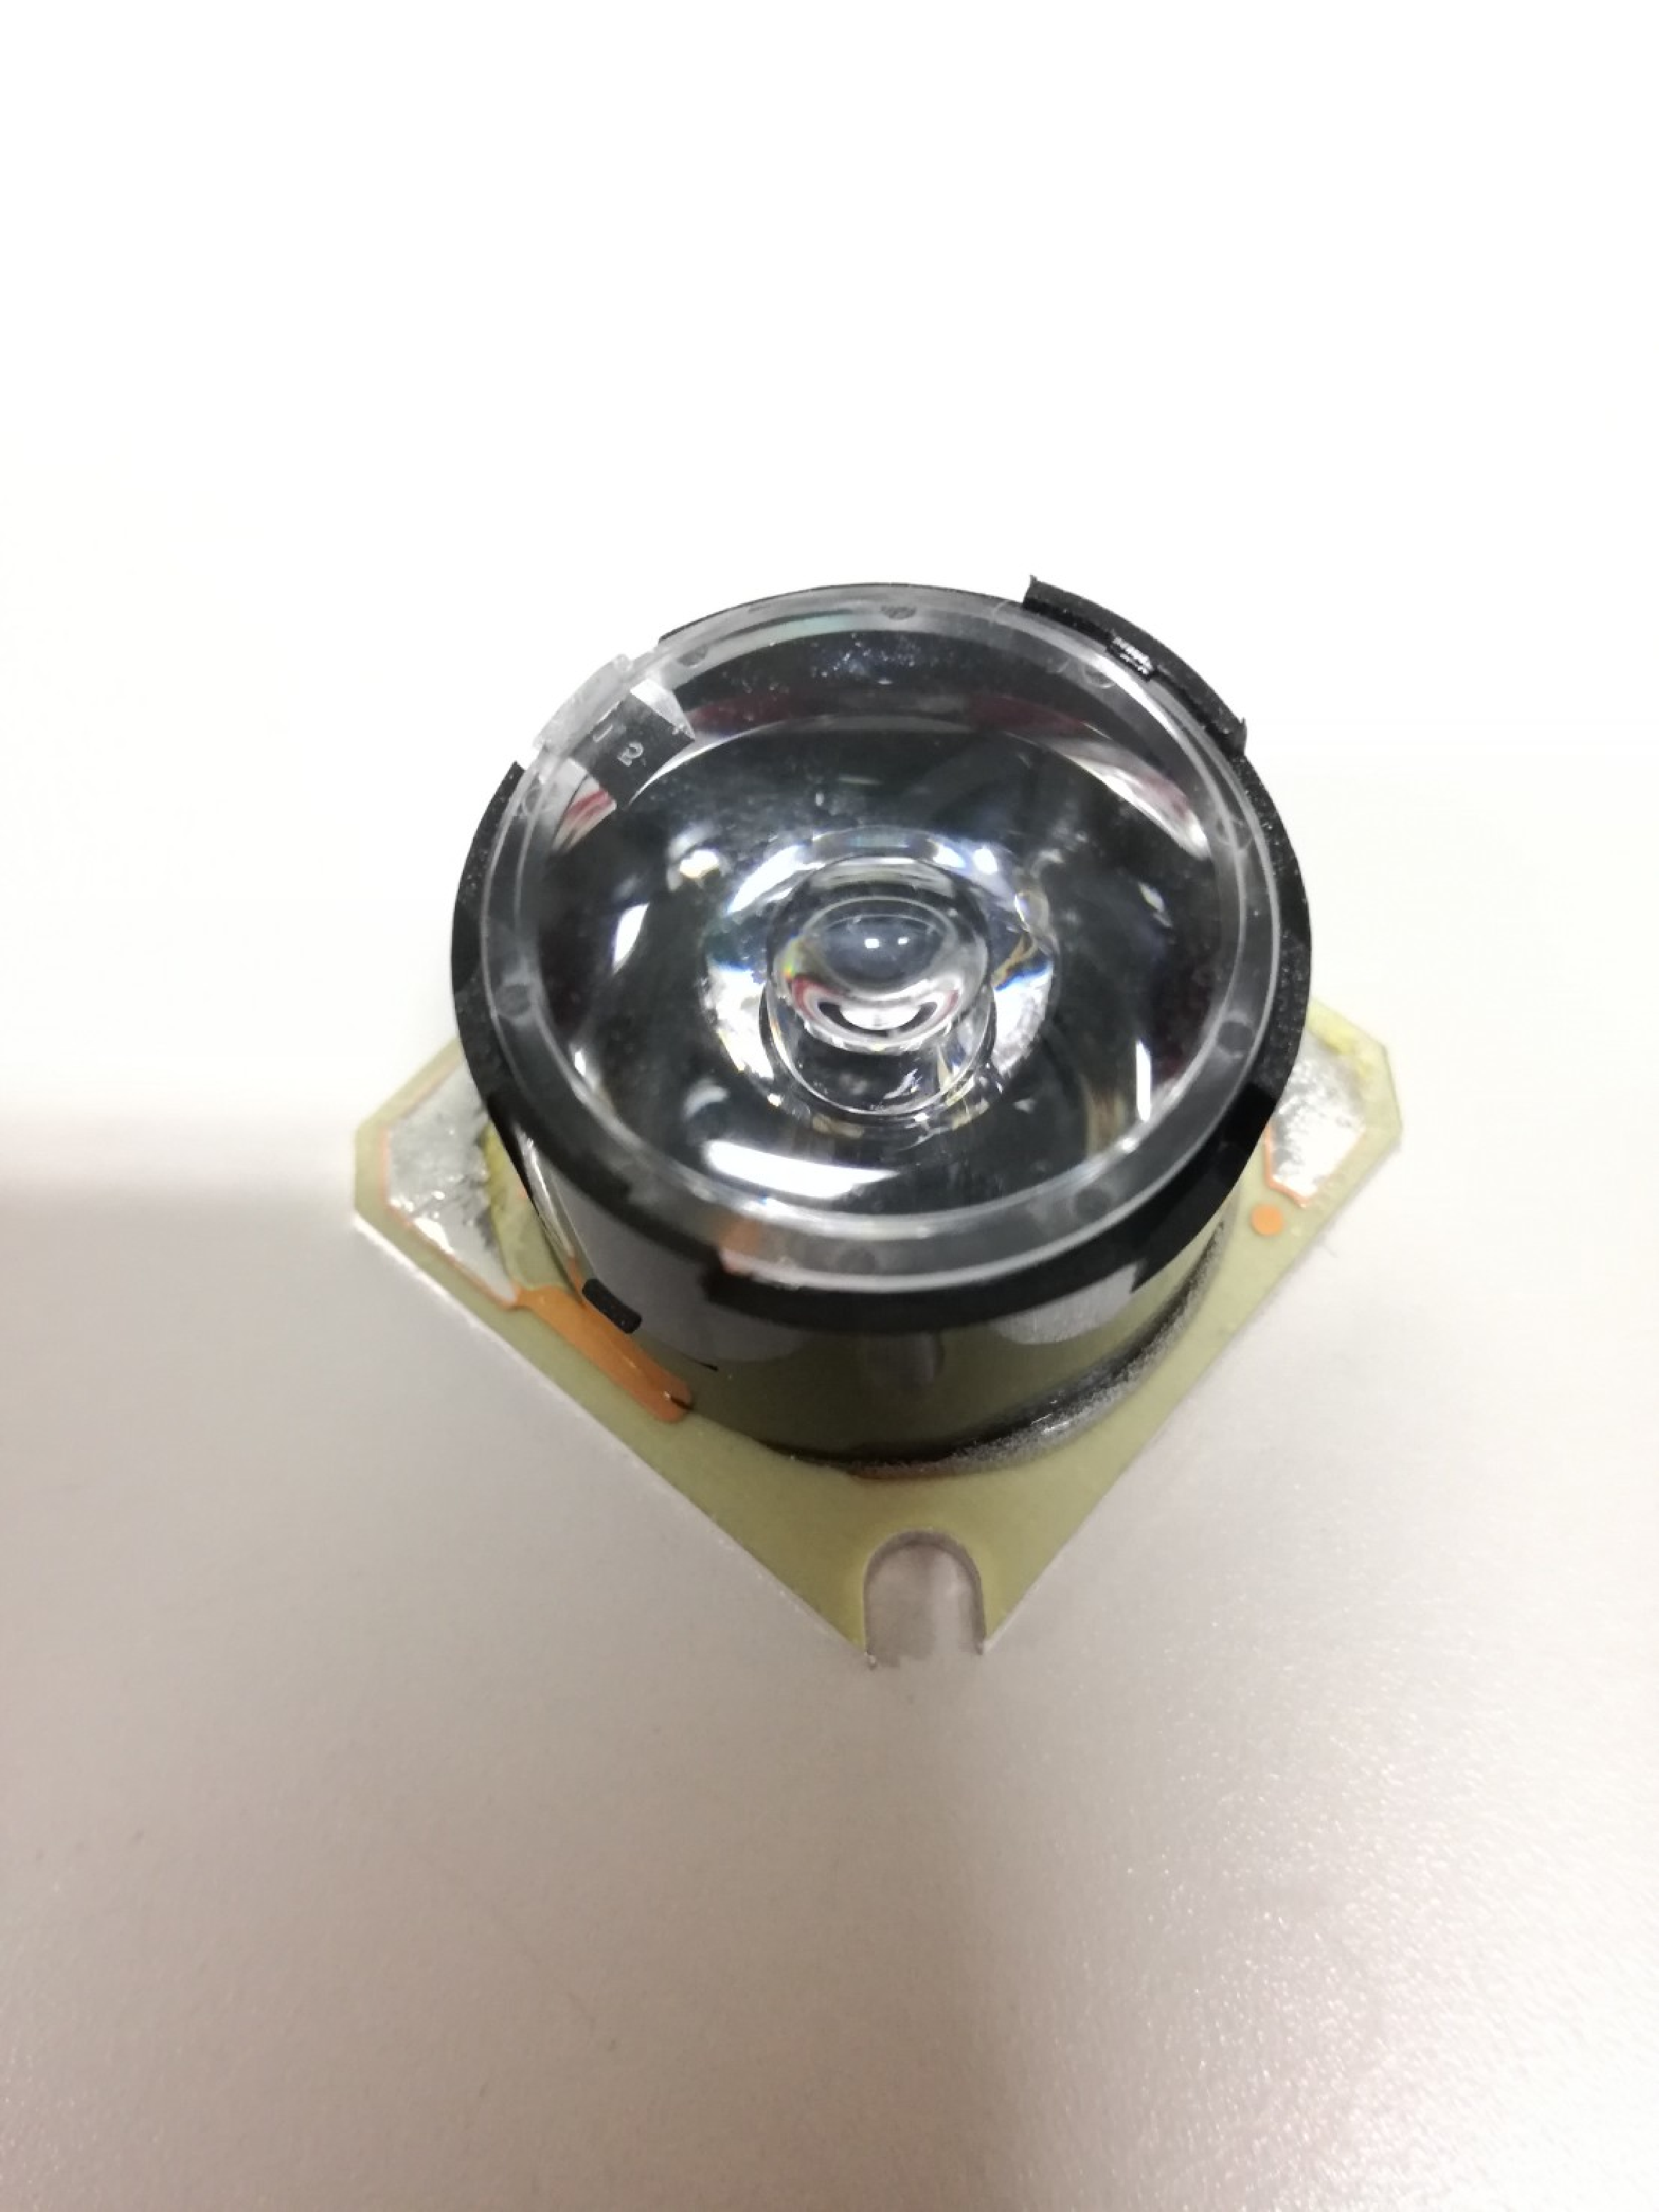
\includegraphics[width=40mm]{fig/led.pdf}
  \end{center}
  \caption{LED}
   \figlab{led}
 \end{minipage}
 \begin{minipage}{0.5\hsize}
 \begin{center}
  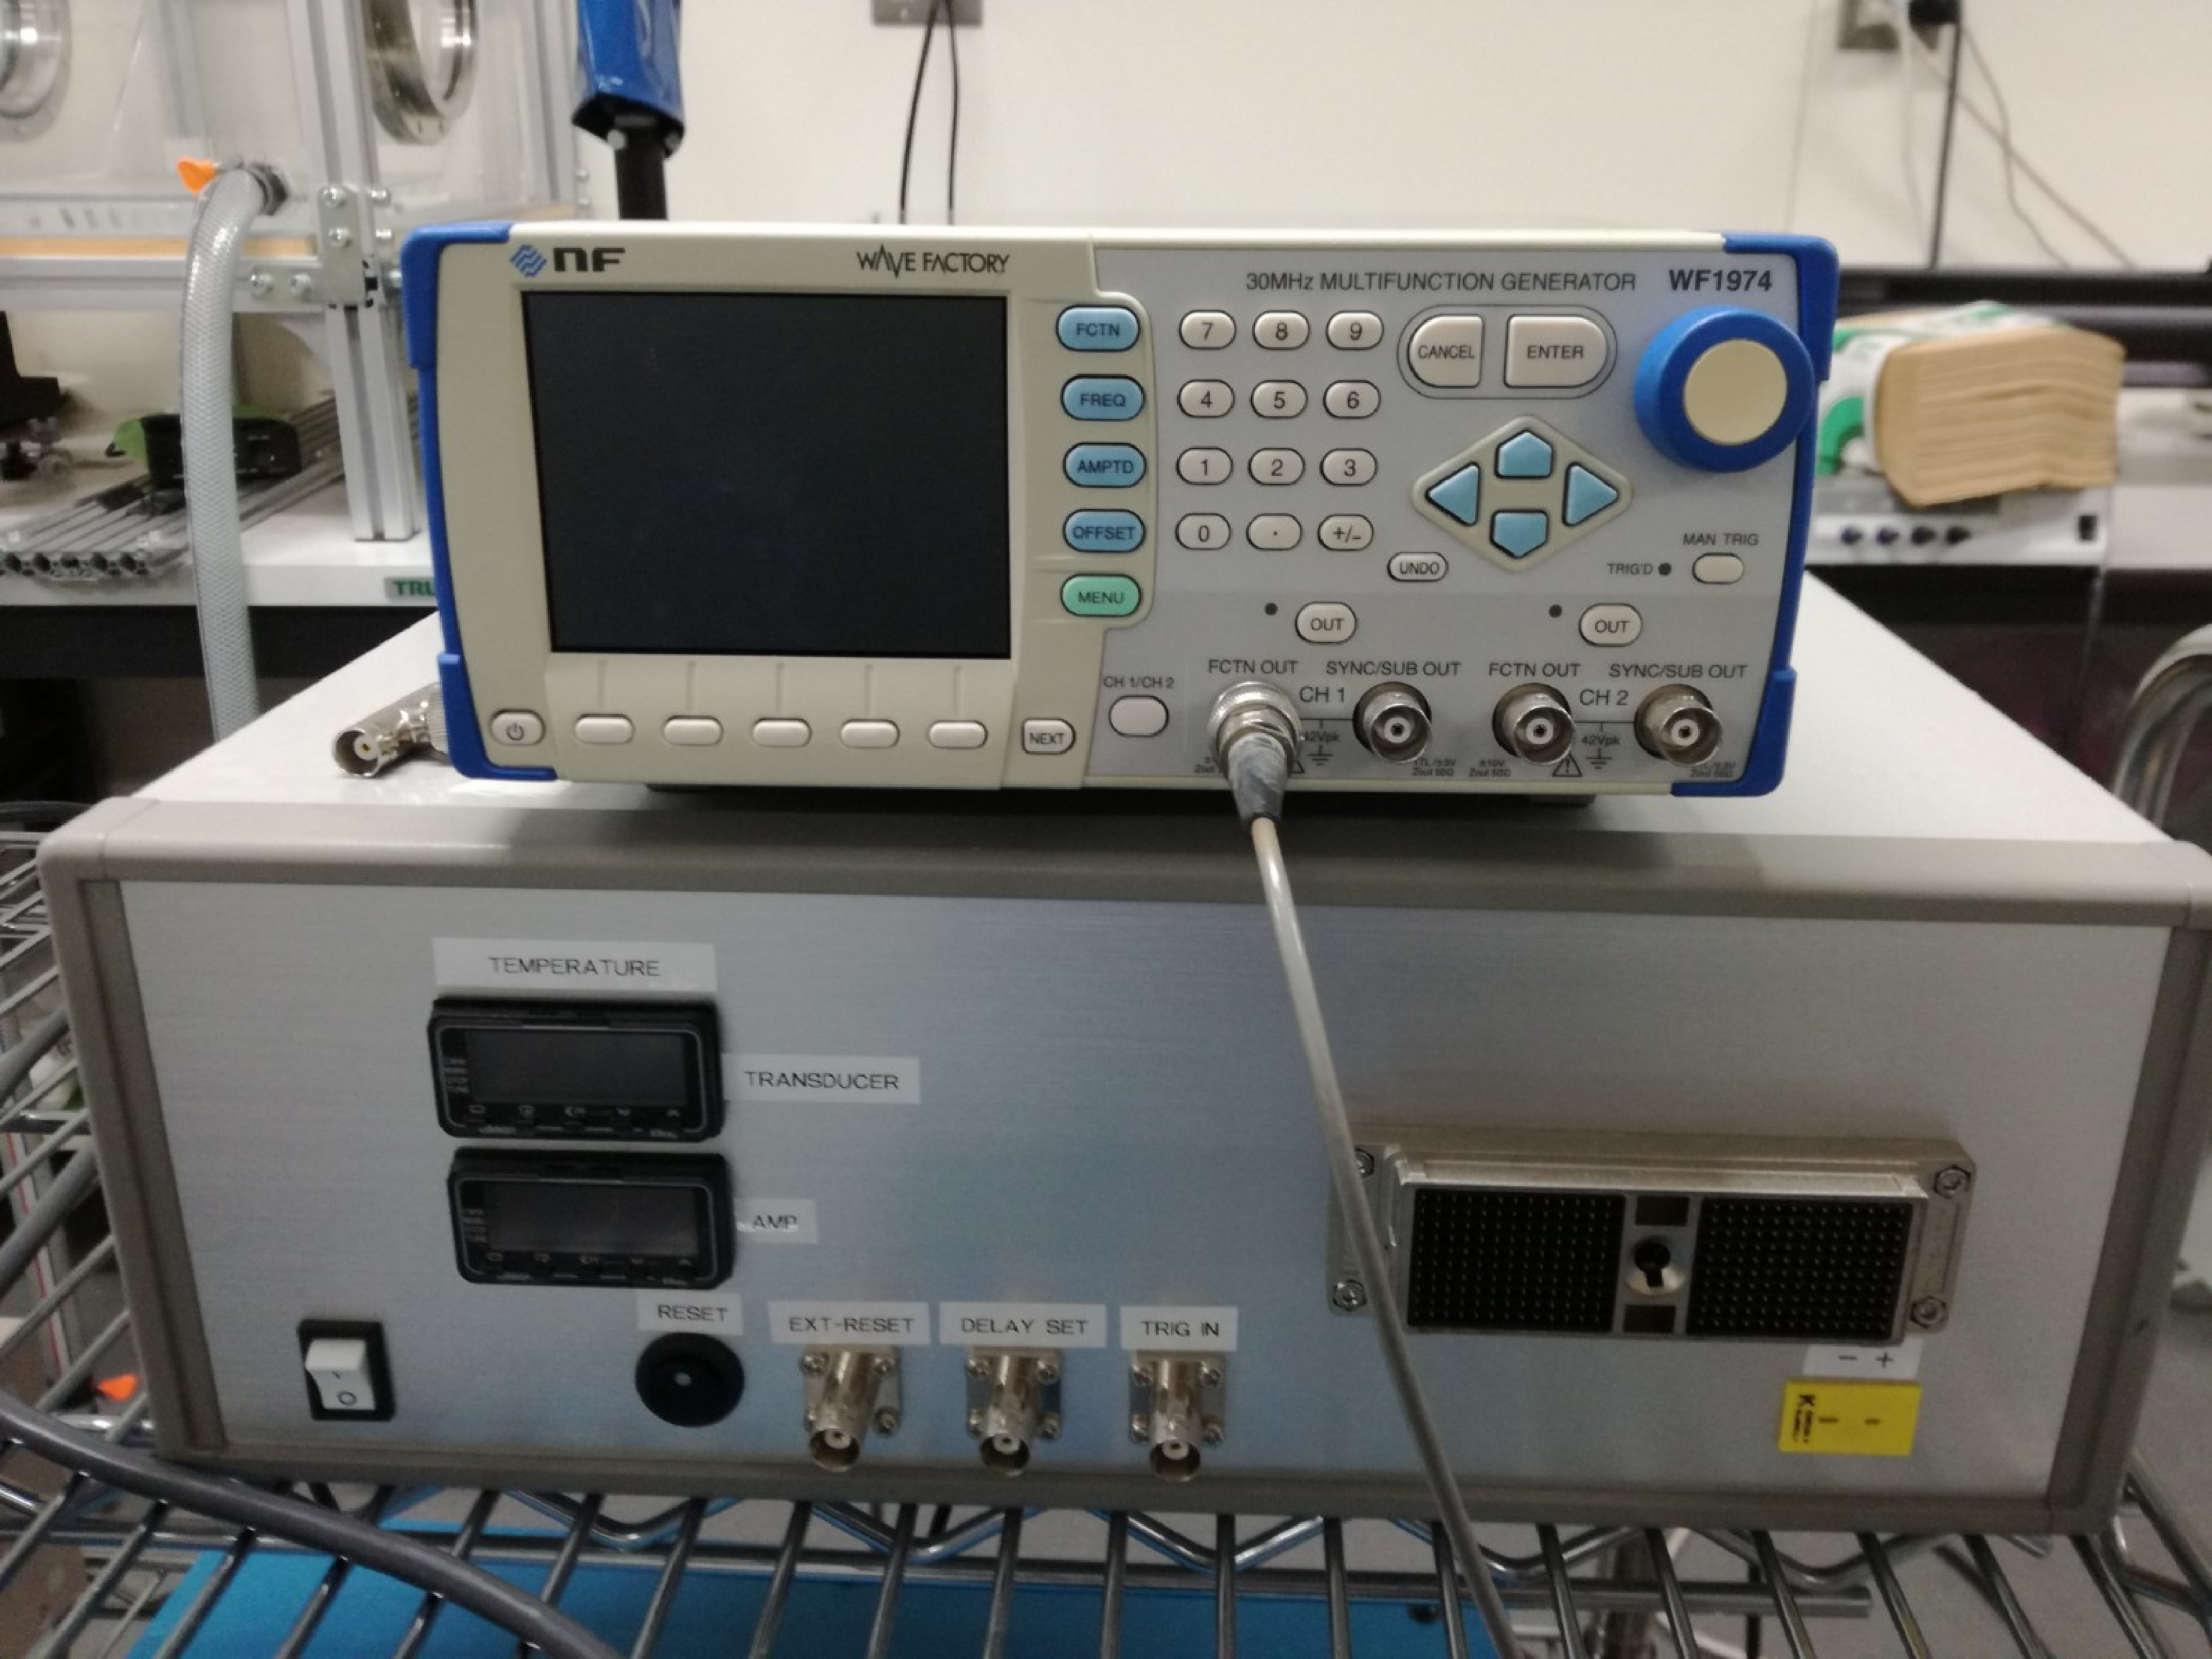
\includegraphics[width=70mm]{fig/fanction.pdf}
 \end{center}
  \caption{ファンクションジェネレータ }
  \figlab{fanction}
 \end{minipage}
\end{figure}
%\end{itemize}
%\begin{figure}[H]
%  \begin{center}
%   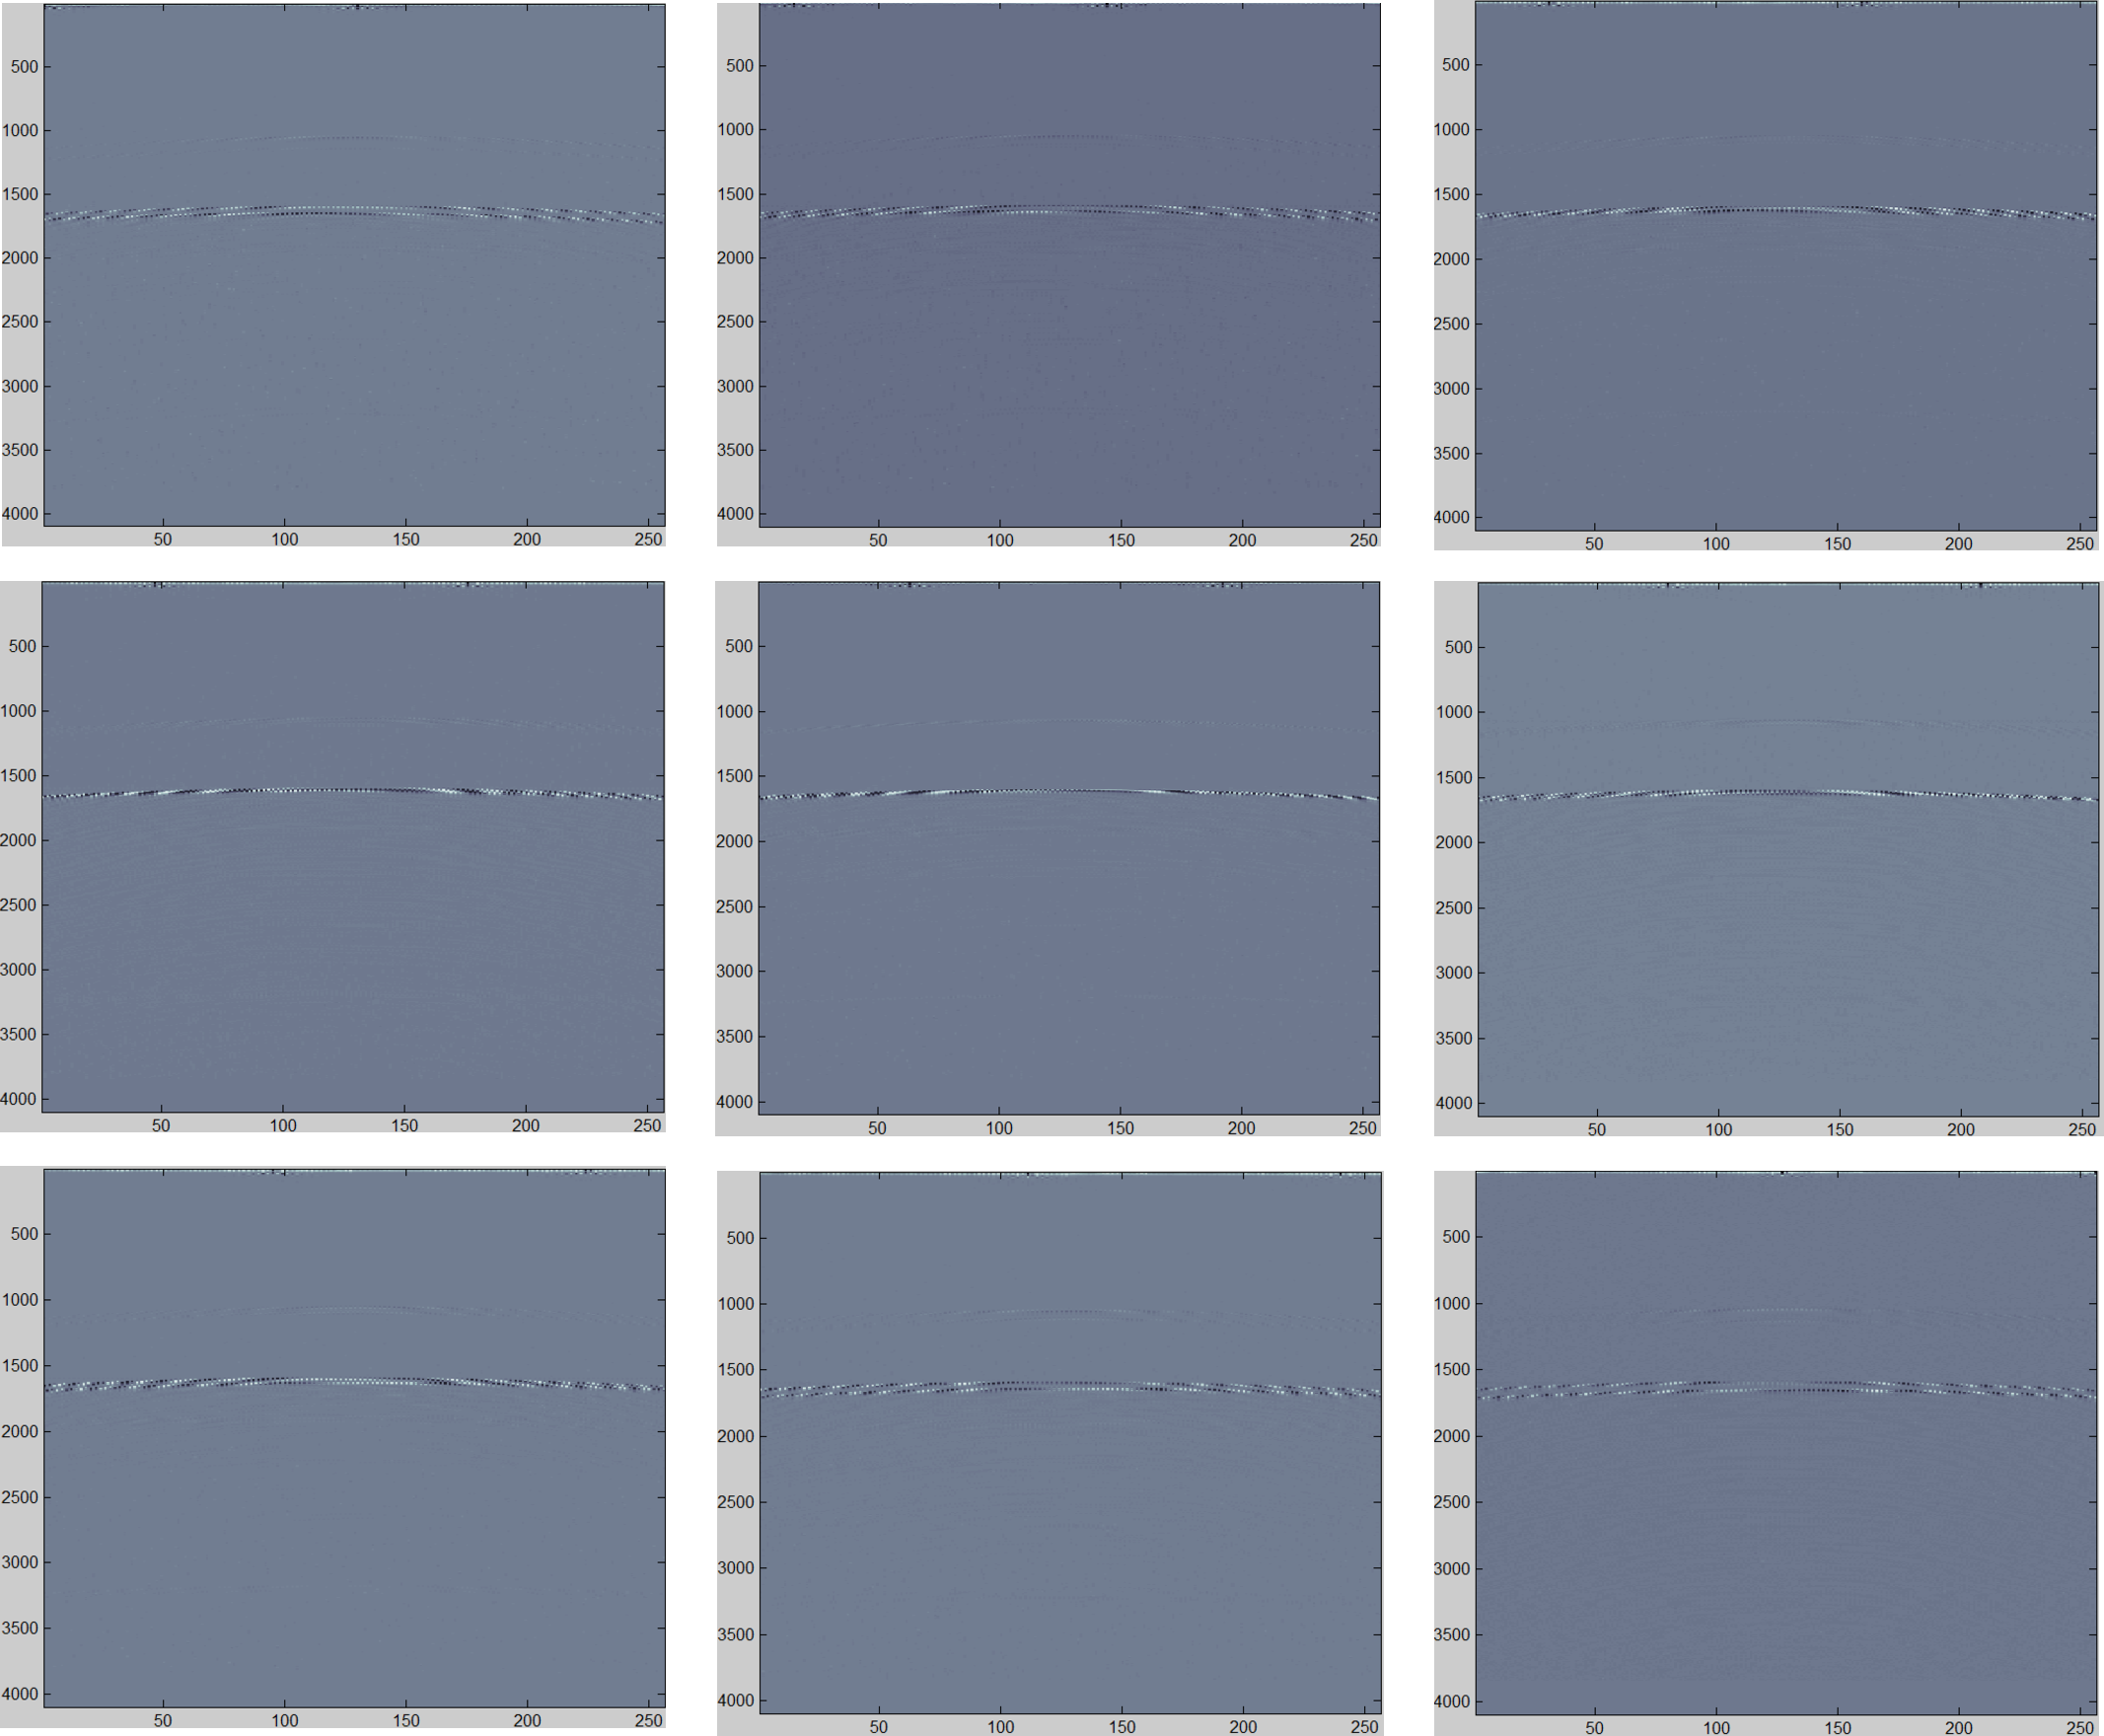
\includegraphics[width=140mm]{fig/1210seishi_denpan.pdf}
%  \end{center}
%  \caption{平面波入射時の各送信条件における受信素子と時間の関数}
%  \figlab{1210seishi_denpan}
%\end{figure}
\subsection{実験手順}
本研究における実験手順を下記に示す. 詳細な手順, 実験手順については各章を参照されたい. 
\begin{enumerate}
  \item 水槽に水を入れ, 振動装置を治具に固定する. この際に, 水槽の水の温度を測定する. 
  %脱気とか必要なのか
  \item ファントムについては, 釣り糸, 水糸, 鶏の腱の3種類を用意した. 鶏の腱については, 実験前日などに新鮮な状態のものを入手する. 
  \item 振動時の弦の撮像のためのカメラを設置する. 
  %鶏の腱を用いるかどうかはまた後で考える
  \item ファントムを適切な長さに切り出し, 振動装置に固定する. 
  \item Verasonicsとコネクタで繋がれたプローブを治具に固定して, 水槽内に入れる. プローブ表面に気泡が付着することがあるので, 取り除く. 
  %気泡の取り除き方?
  \item PCを起動することで, Verasonicsも同時に起動する. 撮像条件は, Matlab上で調整する. 実験条件に合わせてプログラムを実行する. 超音波診断装置の撮像開始トリガーはVerasonicsと接続されたPCで操作するので, FGからエコーへの入力開始と同時にVerasonicsも撮像を開始する.
   %吉村さんP47
   \item まずは, 静止状態での弦に超音波を入射させ, RcvDataデータを取得する. その後, リアルタイムでの撮像が可能プログラムで, 静止状態の弦の画像をキャプチャして, 後述する再構成画像との比較の際の資料とする. 
   \item カメラで振動の撮像を開始する. 
   \item 振動時の弦に超音波を入射させる. 使用する振動モータの周波数に合わせて撮像時間を調整し, RFデータの時間変化を含んだRcvDataを取得する. 
   \item プローブの固定角度を変えて, 1.\verb|〜|7. の過程を繰り返す.
   \item 振動モータは電圧で駆動しているが, 電圧を調整し振動数を変え, 1.\verb|〜|7. の過程を繰り返す.
   \item ファントムの長さを変えて, 1.\verb|〜|11. の過程を繰り返す.
   \item FGおよび電圧の電源を落とす. 
   \item プローブ, 振動装置, 治具を水槽内から取り除く. 
   \item 水槽の水を捨て, 水槽を洗浄する. この際に水槽の水の温度を測る.    
\end{enumerate}

